\chapter{B Chapter}

\lipsum[1] \ref{fig:frogger}\ref{fig:froggerr}.

\begin{figure}
    \centering
    \caption{\label{fig:frogger}Another instance of the frog.}
    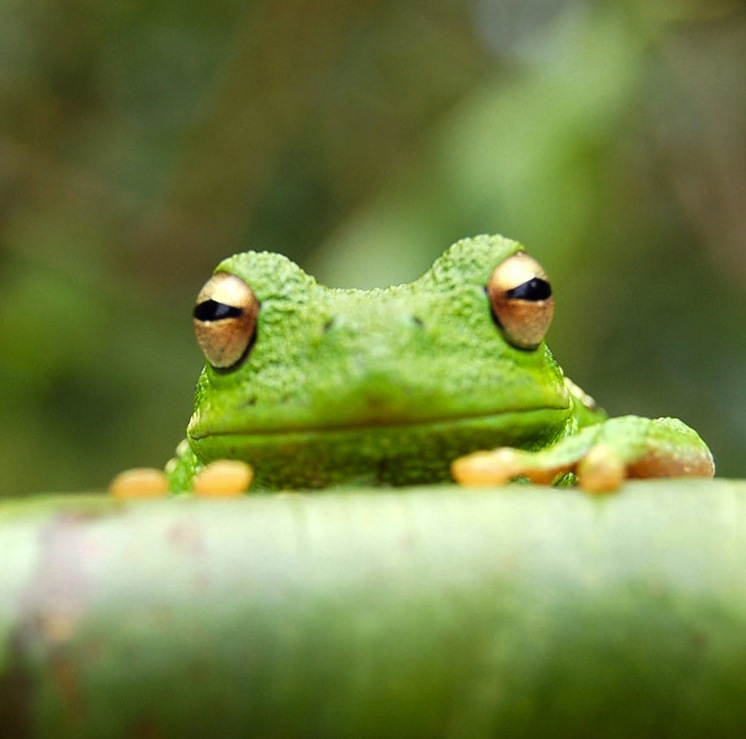
\includegraphics[width=0.3\textwidth]{frog.jpg}
\end{figure}
\begin{figure}
    \centering
    \caption{\label{fig:froggerr}And a third one.}
    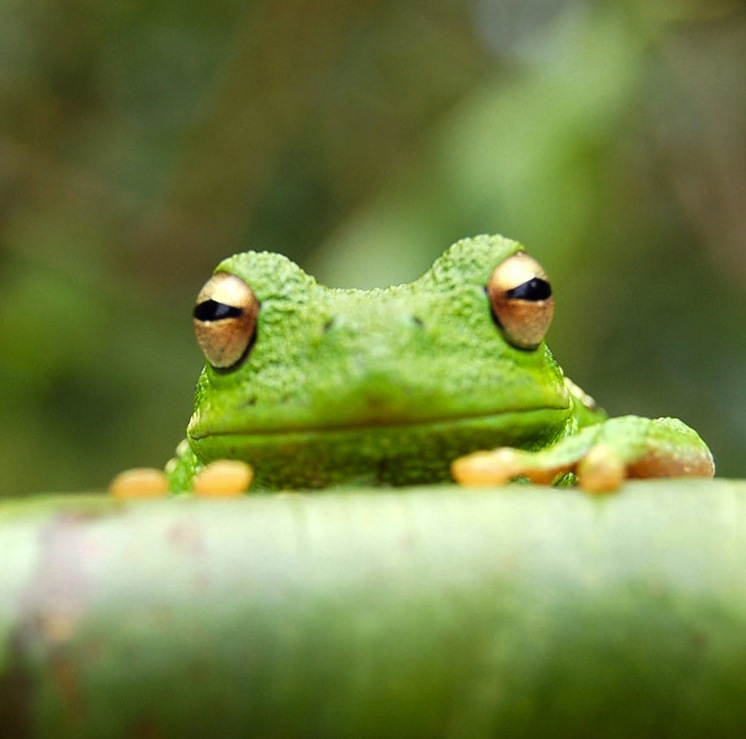
\includegraphics[width=0.3\textwidth]{frog.jpg}
\end{figure}

\section{A Section}

\lipsum[2]

\section{B Section}

\subsection{A Subsection}
\lipsum[3]
\subsubsection{A Subsubsection}
\lipsum[4]
\subsection{B subsection}
\lipsum[5]

\section{C Section}
\lipsum[6-8] \ref{tab:widgetss} \cite{One, Two, Three}.

\begin{table}
    \centering
    \caption{\label{tab:widgetss}An example table.}
    \begin{tabular}{l|r}
        Item & Quantity \\\hline
        Widgets & 42 \\
        Gadgets & 13
    \end{tabular}
\end{table}

\begin{enumerate}
\item first,
\item second.
\end{enumerate}
\dots and bullet points \dots
\begin{itemize}
\item one bullet,
\item two bullets.
\end{itemize}

Let $X_1, X_2, \ldots, X_n$ be a sequence of independent and identically distributed random variables with $\text{E}[X_i] = \mu$ and $\text{Var}[X_i] = \sigma^2 < \infty$, and let
\[S_n = \frac{X_1 + X_2 + \cdots + X_n}{n}
      = \frac{1}{n}\sum_{i}^{n} X_i\]
denote their mean. Then as $n$ approaches infinity, the random variables $\sqrt{n}(S_n - \mu)$ converge in distribution to a normal $\mathcal{N}(0, \sigma^2)$.

\begin{quote}
    \lipsum[10]
\end{quote}